%% LaTeX-Beamer template for KIT design
%% by Erik Burger, Christian Hammer
%% title picture by Klaus Krogmann
%%
%% version 2.1
%%
%% mostly compatible to KIT corporate design v2.0
%% http://intranet.kit.edu/gestaltungsrichtlinien.php
%%
%% Problems, bugs and comments to
%% burger@kit.edu

\documentclass[18pt]{beamer}

%% SLIDE FORMAT

% use 'beamerthemekit' for standard 4:3 ratio
% for widescreen slides (16:9), use 'beamerthemekitwide'
% for widescreen slide without sidebar use 'beamerthemekitwidenosidebar'

\usepackage{templates/beamerthemekit}
%\usepackage{templates/beamerthemekitwide}
%\usepackage{templates/beamerthemekitwidenosidebar}

% use this to disable the latex beamer navigation symbols
\beamertemplatenavigationsymbolsempty


%% TITLE PICTURE

% if a custom picture is to be used on the title page, copy it into the 'logos'
% directory, in the line below, replace 'mypicture' with the 
% filename (without extension) and uncomment the following line
% (picture proportions: 63 : 20 for standard, 169 : 40 for wide
% *.eps format if you use latex+dvips+ps2pdf, 
% *.jpg/*.png/*.pdf if you use pdflatex)

\titleimage{GoodWillHunting.jpg}

%% TITLE LOGO

% for a custom logo on the front page, copy your file into the 'logos'
% directory, insert the filename in the line below and uncomment it

\titlelogo{Graph_K3_3.svg.png}

% (*.eps format if you use latex+dvips+ps2pdf,
% *.jpg/*.png/*.pdf if you use pdflatex)

%% TikZ INTEGRATION

% use these packages for PCM symbols and UML classes
% \usepackage{templates/tikzkit}
% \usepackage{templates/tikzuml}

% the presentation starts here

\title[IMP]{IMP}
\subtitle{Informatik, Mathematik, Physik}
\author{Malte Vo\ss}

\institute{Abteilung für Didaktik der Mathematik}

\date{29. Januar 2020}

% Bibliography

\usepackage{babelbib}
\bibliographystyle{babplain-lf}

\begin{document}

% change the following line to "ngerman" for German style date and logos
\selectlanguage{ngerman}

%title page
\begin{frame}
\titlepage
\end{frame}

%table of contents
\begin{frame}{Gliederung}
\tableofcontents
\end{frame}

\section{Profilfach IMP}
    \subsection{Lehrplan}
    \begin{frame}{Example slide A}
    \begin{itemize}
    \item
    \pause
    \item Bullet point 2
    \item \dots
    \end{itemize}
    \end{frame}

    \subsection{Subsection 1.2}
    \begin{frame}{Example slide B}
    \begin{block}{Block 1}
    \begin{itemize}
    \item Bullet point 1
    \pause
    \item Bullet point 2
    \item \dots
    \end{itemize}
    \end{block}
    \end{frame}

\section{Graphen}
    \begin{frame}{Was sind Graphen?}
        \begin{block}{Formale Definition}
            \glqq Ein gerichteter Graph ist festgelegt durch ein Paar $G = (V, E)$, wobei $E \subset V \times V$ ist\grqq \cite{worsch2016}.
        \end{block}
        \pause
        \begin{block}{etwas handlicher}
            Ein Graph besteht aus Knoten und Kanten, wobei jede Kante zwei Knoten verbindet.
        \end{block}
        \pause
        \begin{block}{etwas mathematischer}
            Ein Graph stellt eine Relation zwischen Objekten dar.
        \end{block}
    \end{frame}

    \begin{frame}[allowframebreaks]{Wozu benutzt man Graphen?}
        \begin{block}{Ein paar Beispiele}
            \begin{itemize}[<+->]
                \item Straßennetz modellieren
                \item Abläufe modellieren
                \item Navigationssysteme
                \item Automaten darstellen
                \item Soziale Netzwerke
                \item Maschinelles Lernen
                \item \dots
            \end{itemize}
        \end{block}
        \begin{figure}[]
            \centering
            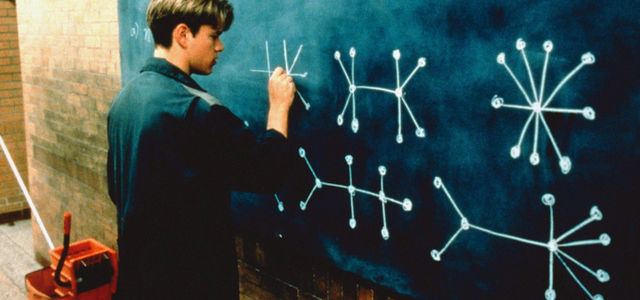
\includegraphics[keepaspectratio,width=\textwidth]{logos/GoodWillHunting.jpg}
            \caption{Good Will Hunting, Gus Van Sant 1997}
        \end{figure}
    \end{frame}

    \begin{frame}{Das Haus vom Nikolaus}
        \begin{align*}
            V & := \{1, \dots, 5\}
            \\
            E & := \bigl\{ \{1,2\}
                         , \{1,5\}
                         , \{2,3\}
                         , \{2,4\}
                         , \{2,5\}
                         , \{3,4\}
                         , \{3,5\}
                         , \{4,5\}
                   \bigr\}
        \end{align*}

        \pause

        \begin{figure}[h]
            \centering
            \begin{tikzpicture}
                \begin{scope}[color=black]
                \draw[fill] (0,0) circle (2pt);
                \draw[fill] (1,0) circle (2pt);
                \draw[fill] (0,1) circle (2pt);
                \draw[fill] (0.5,1.5) circle (2pt);
                \draw[fill] (1,1) circle (2pt);
                \end{scope}
                \begin{scope}[color=blue]
                \draw (0.5,1.5) node[above] {$1$};
                \draw (1,1) node[right] {$2$};
                \draw (1,0) node[right] {$3$};
                \draw (0,0) node[left] {$4$};
                \draw (0,1) node[left] {$5$};
                \end{scope}
                \draw[-,rounded corners=0.1cm]
                (0,0) -- (1,0) -- (0,1) -- (1,1) -- (0,0)
                -- (0,1) -- (0.5,1.5) -- (1,1) -- (1,0);
            \end{tikzpicture}
            \caption{Das Haus vom Nikolaus}
            \label{fig:hausvomnikolaus}
        \end{figure}
    \end{frame}

    \begin{frame}[allowframebreaks]{Königsberger Brückenproblem}
        \begin{figure}
            \centering
            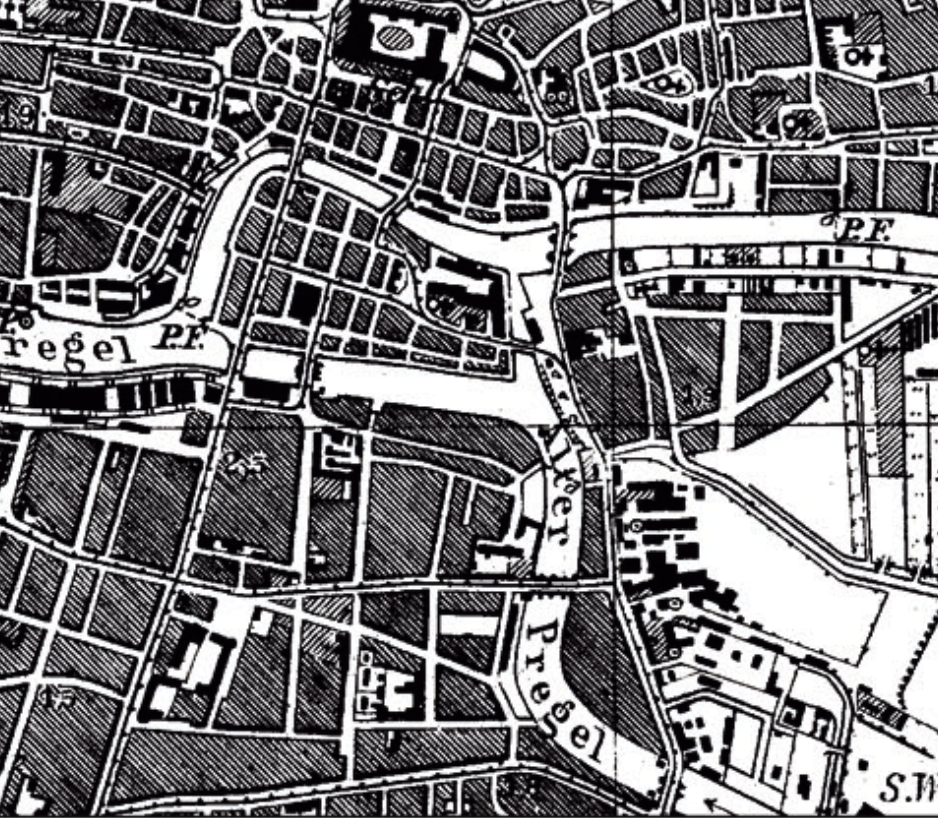
\includegraphics[keepaspectratio,width=180px]{figures/Konigsberg_Brucken_BKG.png}
            \caption{Königsberg 1937 \cite{bkg_kon}}
        \end{figure}

        \framebreak

        \begin{figure}
            \centering
            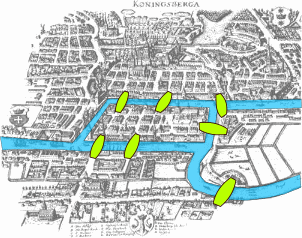
\includegraphics[keepaspectratio,height=130px]{figures/Konigsberg_bridges.png}
            \caption{\tiny \url{wikimedia.org}}
            \glqq Die Einwohner fragten sich, ob es möglich sei, durch die Stadt zu spazieren und dabei alle Brücken genau einmal zu überqueren.\grqq
        \end{figure}
    \end{frame}

    \begin{frame}{}
        \begin{figure}[]
            \centering
            \begin{tikzpicture}
                \node (a) at (0,4) {$a$};
                \node (b) at (0,2) {$b$};
                \node (c) at (0,0) {$c$};
                \node (d) at (4,2) {$d$};
          
                \foreach \from/\to/\pos in {a/b/20,a/b/-20,a/d/0,b/c/20,b/c/-20,b/d/0,c/d/0}
                  \draw[line width=2pt] (\from) to [bend left=\pos] (\to);
            \end{tikzpicture}  
            \caption{Königsberg als Graph}
        \end{figure}  
    \end{frame}

\subsection{Planare Graphen}
% Satz von Kuratowski
% K_{3,3} Versorger-Verbraucher-Problem

\section{Videos}
    \begin{frame}{Graphen und Euler-Characteristik}
        Was ist die Euler-Characteristik?

        \url{https://www.youtube.com/watch?v=-9OUyo8NFZg}
    \end{frame}

    \appendix
    \beginbackup

    \begin{frame}[allowframebreaks]{Quellen}
    \bibliography{references}
    \end{frame}

    \backupend

\end{document}
